% Formulario TEEA 3MAT — Argomento 1: tensione, corrente, resistenza e legge di Ohm
% Per rigenerare il PDF (dalla cartella strumenti, due volte per il numero di pagine):
%   pdflatex -output-directory=../pdf -jobname=01-formulario-tensione-corrente-resistenza formulario.tex
% ---------------------------------------------------------------------------
%  Stile comune dei formulari TEEA (pdfLaTeX, solo pacchetti standard
%  presenti in TeX Live e MiKTeX). Testo in Computer Modern Sans.
% ---------------------------------------------------------------------------
\documentclass[11pt,a4paper]{article}
\usepackage[a4paper, top=14mm, bottom=16mm, left=14mm, right=14mm, headheight=0pt, footskip=8mm]{geometry}
\usepackage[utf8]{inputenc}
\usepackage{amsmath, amssymb}
\renewcommand{\familydefault}{\sfdefault}
\newcommand{\ohm}{\ensuremath{\Omega}}
\newcommand{\uA}{\ensuremath{\mu}}
\newcommand{\per}{\ensuremath{\cdot}}
\usepackage{xcolor, tikz, multicol, booktabs, array, fancyhdr, lastpage, tabularx}
\usepackage[most]{tcolorbox}
\usetikzlibrary{arrows.meta}

\definecolor{verde}{HTML}{159957}
\definecolor{blu}{HTML}{155799}
\definecolor{inchiostro}{HTML}{1B2936}
\definecolor{tenue}{HTML}{606C71}
\definecolor{fondo}{HTML}{EEF3F0}
\definecolor{tensione}{HTML}{2152C0}
\definecolor{corrente}{HTML}{B3205F}
\definecolor{resistenza}{HTML}{0B7A62}
\color{inchiostro}

\setlength{\parindent}{0pt}
\setlength{\columnsep}{7mm}
\renewcommand{\arraystretch}{1.25}

% unità di misura in tondo e virgola decimale
\newcommand{\U}[1]{\,\mathrm{#1}}
\newcommand{\virg}{{,}}

% riquadro di un argomento
\newtcolorbox{blocco}[1]{enhanced, breakable=false, colback=white, colframe=verde, boxrule=0.6pt,
  leftrule=3pt, arc=1.5pt, left=6pt, right=6pt, top=4pt, bottom=5pt,
  title={\bfseries #1}, coltitle=verde, colbacktitle=fondo, fonttitle=\normalsize,
  toptitle=1pt, bottomtitle=1pt, before skip=0pt, after skip=4.5mm}

% formula grande centrata
\newcommand{\F}[1]{\par\smallskip{\centering\Large$\displaystyle #1$\par}\smallskip}
% legenda dei simboli
\newcommand{\leg}[1]{{\small\color{tenue}#1}\par}

% intestazione del formulario
\newcommand{\intestazione}[3]{%
  {\color{verde}\bfseries\small #1}\par\vspace{1mm}
  {\fontsize{19}{23}\selectfont\bfseries #2}\par\vspace{1mm}
  {\small\color{tenue} #3}\par\vspace{2mm}
  {\color{verde}\rule{\linewidth}{1.6pt}}\par\vspace{4mm}}

\pagestyle{fancy}
\fancyhf{}
\renewcommand{\headrulewidth}{0pt}
\fancyfoot[L]{\scriptsize\color{tenue}Prof. Pasquale Naclerio \per{} TEEA 3MAT \per{} Formulario}
\fancyfoot[R]{\scriptsize\color{tenue}Pagina \thepage\ di \pageref{LastPage}}

\begin{document}

\intestazione{TEEA --- 3MAT \per{} Argomento 1 \per{} FORMULARIO}
             {Tensione, corrente, resistenza e legge di Ohm}
             {Prof. Pasquale Naclerio \per{} Manutenzione e Assistenza Tecnica}

\begin{blocco}{Grandezze elettriche fondamentali}
\begin{tabularx}{\linewidth}{@{}l c l l X@{}}
\toprule
\textbf{Grandezza} & \textbf{Simbolo} & \textbf{Unità} & \textbf{Strumento} & \textbf{Collegamento}\\
\midrule
\color{tensione}tensione   & \color{tensione}$V$   & volt (V)    & voltmetro   & in parallelo al componente\\
\color{corrente}corrente   & \color{corrente}$I$   & ampere (A)  & amperometro & in serie al componente\\
\color{resistenza}resistenza & \color{resistenza}$R$ & ohm (\ohm)   & ohmmetro    & sul componente scollegato\\
\bottomrule
\end{tabularx}
\end{blocco}

\begin{multicols}{2}

\begin{blocco}{Legge di Ohm}
\begin{minipage}[c]{0.6\linewidth}
\F{V = R \cdot I}
\F{I = \frac{V}{R}}
\F{R = \frac{V}{I}}
\end{minipage}\hfill
\begin{minipage}[c]{0.36\linewidth}\centering
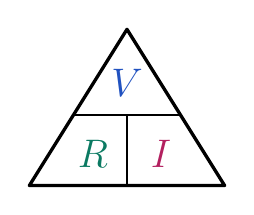
\begin{tikzpicture}[scale=0.62, line join=round]
  \draw[line width=1.2pt] (0,0) -- (4,0) -- (2,3.2) -- cycle;
  \draw[line width=0.9pt] (0.9,1.45) -- (3.1,1.45) (2,0) -- (2,1.45);
  \node[tensione, font=\Large\bfseries] at (2,2.1) {$V$};
  \node[resistenza, font=\Large\bfseries] at (1.3,0.65) {$R$};
  \node[corrente, font=\Large\bfseries] at (2.7,0.65) {$I$};
\end{tikzpicture}
\end{minipage}
\leg{$V$ [V] \quad $I$ [A] \quad $R$ [\ohm]}
\end{blocco}

\begin{blocco}{Intensità di corrente}
\F{I = \frac{Q}{t}}
\leg{$Q$ carica [C] \quad $t$ tempo [s] \quad $I$ [A] \qquad $1\U{A} = 1\U{C/s}$}
\end{blocco}

\begin{blocco}{Generatore di tensione}
\textbf{ideale:}
\F{V = E}
\textbf{reale} (resistenza interna $R_i$):
\F{V = E - R_i \cdot I}
\leg{$E$ forza elettromotrice [V] (tensione a vuoto, $I = 0$)}
\end{blocco}

\columnbreak

\begin{blocco}{Resistenza di un filo (seconda legge di Ohm)}
\F{R = \rho \cdot \frac{L}{S}}
\leg{$\rho$ resistività [\ohm\per mm\textsuperscript{2}/m] \quad $L$ lunghezza [m] \quad $S$ sezione [mm\textsuperscript{2}]}
\leg{rame: $\rho \approx 0\virg0175\,\Omega\cdot\mathrm{mm^2/m}$}
\end{blocco}

\begin{blocco}{Coppie di unità comode}
\begin{tabularx}{\linewidth}{@{}X X X@{}}
\toprule
\textbf{Tensione} & \textbf{Resistenza} & \textbf{Corrente}\\
\midrule
V & \ohm & A\\
V & k\ohm & mA\\
\bottomrule
\end{tabularx}
\end{blocco}

\begin{blocco}{Multipli e sottomultipli}
\small
\begin{tabularx}{\linewidth}{@{}l c l X@{}}
\toprule
\textbf{Prefisso} & \textbf{Simbolo} & \textbf{Fattore} & \textbf{Esempio}\\
\midrule
mega  & M & $10^{6}$  & $1\U{M\Omega} = 10^6\U{\Omega}$\\
kilo  & k & $10^{3}$  & $4\virg7\U{k\Omega} = 4700\U{\Omega}$\\
milli & m & $10^{-3}$ & $20\U{mA} = 0\virg02\U{A}$\\
micro & \uA & $10^{-6}$ & $500\,\mu\mathrm{A} = 0\virg0005\U{A}$\\
\bottomrule
\end{tabularx}
\end{blocco}

\end{multicols}

\begin{blocco}{Resistenze in serie e in parallelo}
\begin{minipage}[t]{0.47\linewidth}
\textbf{serie} (stessa corrente):
\F{R_{eq} = R_1 + R_2 + R_3 + \dots}
\F{V = V_1 + V_2 + V_3 + \dots}
\leg{$R_{eq}$ è più grande della resistenza più grande}
\end{minipage}\hfill
\begin{minipage}[t]{0.49\linewidth}
\textbf{parallelo} (stessa tensione):
\F{\frac{1}{R_{eq}} = \frac{1}{R_1} + \frac{1}{R_2} + \frac{1}{R_3} + \dots}
\F{R_{eq} = \frac{R_1 \cdot R_2}{R_1 + R_2} \qquad R_{eq} = \frac{R}{n}}
\F{I = I_1 + I_2 + I_3 + \dots}
\leg{due resistenze \quad / \quad $n$ resistenze uguali $R$; \ $R_{eq}$ è più piccola della più piccola}
\end{minipage}
\end{blocco}


\end{document}
